\subsection{Calorimeter Systems}
\label{sec:calorimeters}

The ATLAS calorimeter systems are situated outside of the ID and central solenoid and
are tasked with the measurement and containment of showers from electrically charged and neutral particles.
A view of the calorimeter systems is provided by Figure~\ref{fig:atlas_calorimeters_cutaway}.
Broadly speaking, there are two types of calorimeters based on their purpose:
electromagnetic and hadronic calorimeters.
The electromagnetic calorimeter system has $\eta$ coverage that matches the inner-detector
and is optimized for precision measurements of electrons and photons.
The hadronic calorimeter system has readout cells that are generally of
coarser grandularity as compared to the electrogmagnetic calorimeter and
is designed to meet the requirements for jet and missing transverse momentum
measurements.
Besides classification by physics purpose, the calorimeter system can also
be broken into two classes based on detector technology: either based
on gaps of cooled liquid-argon~\cite{CERN-LHCC-96-041} or on scintillating tiles as the active media~\cite{CERN-LHCC-96-042}.

\begin{figure}[!htb]
    \begin{center}
        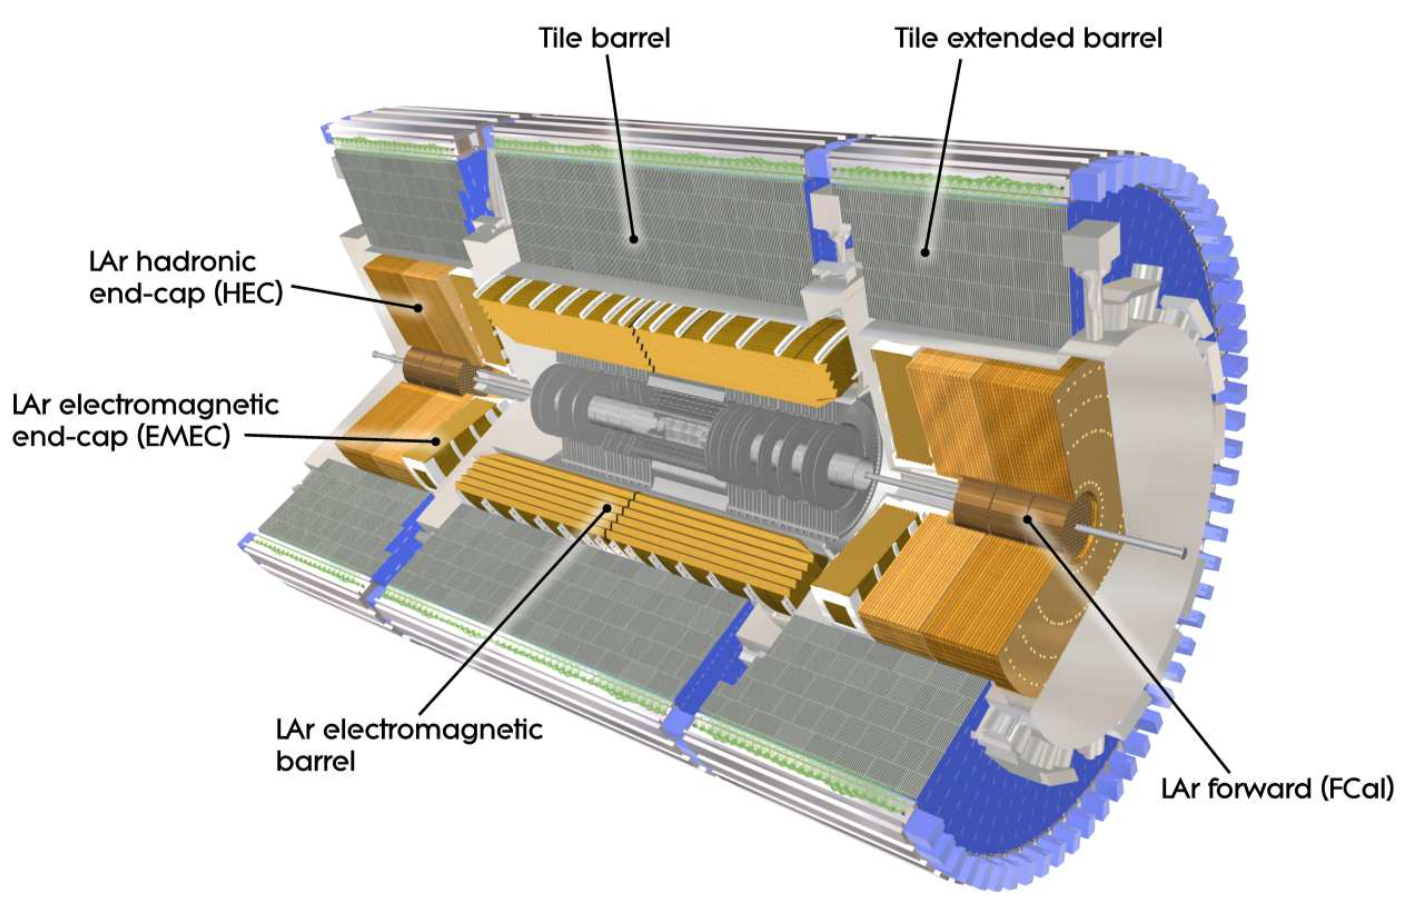
\includegraphics[width=0.9\textwidth]{figures/chapter2/calorimeters/atlas_calorimeter_cutaway}
        \caption{
            Cut-away view of the ATLAS calorimeter system, with liquid-argon and sctintillating-tile
            subsystems indicated.
        }
        \label{fig:atlas_calorimeters_cutaway}
    \end{center}
\end{figure}

\subsubsection{Electromagnetic Calorimeter}
\label{sec:calo_em}

The electromagnetic (EM) calorimeter is a high-granularity lead/liquid-argon (LAr)
sampling calorimeter situated just beyond the central solenoid.
It consists of barrel and end-cap sections, covering the entire
range within $\lvert \eta \rvert < 3.2$, indicated in Figure~\ref{fig:atlas_calorimeters_cutaway}.
The calorimeter is designed in an accordian type structure, whose gaps are
filled with the cooled LAr that acts as the active medium.
The structure of the barrel and end-cap electromagnetic calorimeter
is shown in Figure~\ref{fig:em_calo_section}.
The electromagnetic calorimeter is $>22$ radiation lengths ($X_0$), ensuring
that the majority of electrons and photons are completely contained within the EM calorimeter.
The majority of the EM energy, amounting to approximately 16\,$X_0$, is contained
within the second sampling layer (see Figure~\ref{fig:em_calo_section}).

\begin{figure}[!htb]
    \begin{center}
        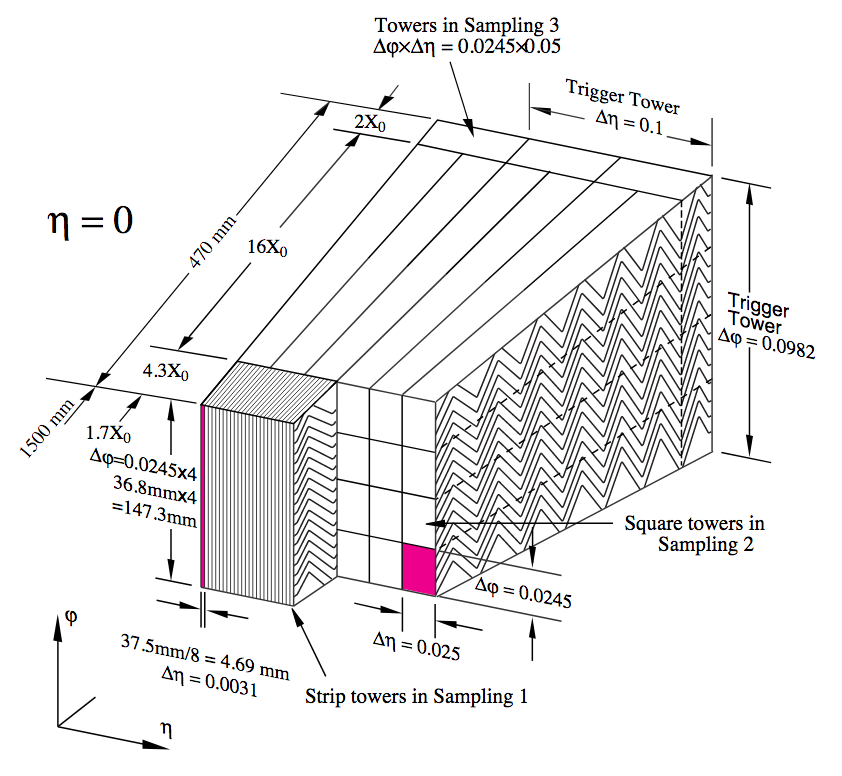
\includegraphics[width=0.6\textwidth]{figures/chapter2/calorimeters/atlas_em_calo_barrel}
        \raisebox{1.5cm}{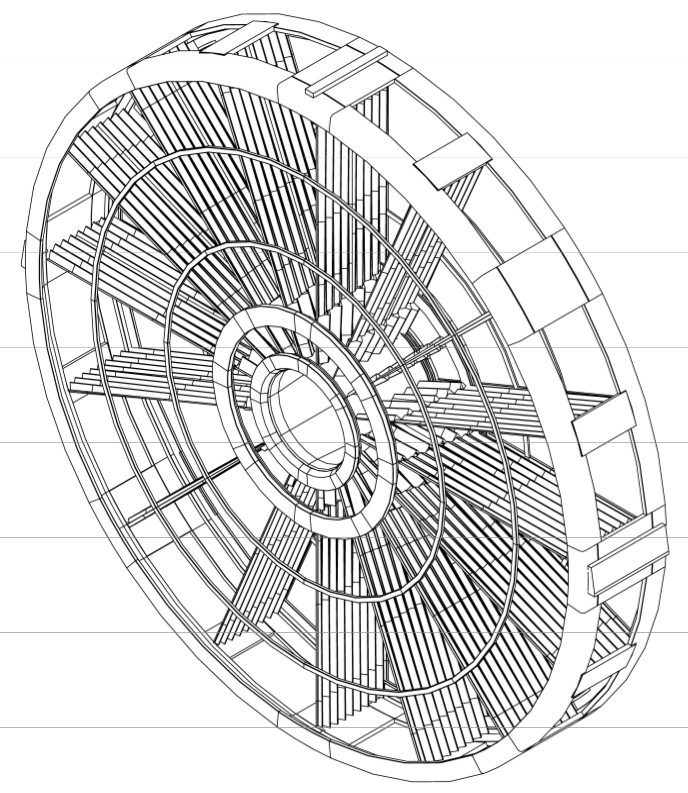
\includegraphics[width=0.3\textwidth]{figures/chapter2/calorimeters/atlas_em_calo_endcap}}
        \caption{
            \textit{Left}: Cut-away view of the barrel electromagnetic calorimeter and its accordian
                structure. Indicated are
                the geometry and absorption properties of the three sampling layers.
            \textit{Right}: Diagram of the electromagnetic end-cap calorimeter accordian wheel structure
                (only a sub-set of the accordian structure is shown).
        }
        \label{fig:em_calo_section}
    \end{center}
\end{figure}

\FloatBarrier
\subsubsection{Hadronic Calorimeter}
\label{sec:calo_had}

\begin{figure}[!htb]
    \begin{center}
        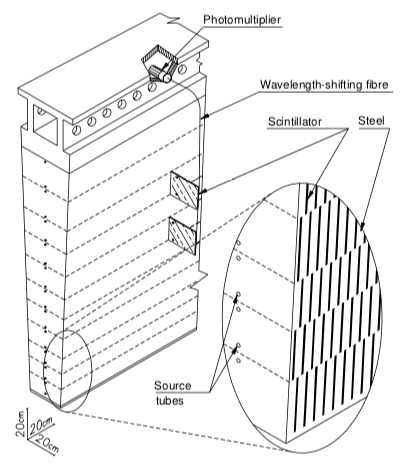
\includegraphics[width=0.4\textwidth]{figures/chapter2/calorimeters/atlas_tile_module}
        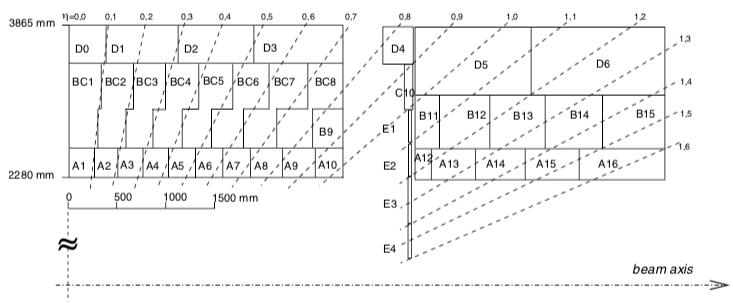
\includegraphics[width=0.9\textwidth]{figures/chapter2/calorimeters/atlas_tile_plan_view}
        \caption{
        }
        \label{fig:tile_calo}
    \end{center}
\end{figure}

\begin{figure}[!htb]
    \begin{center}
        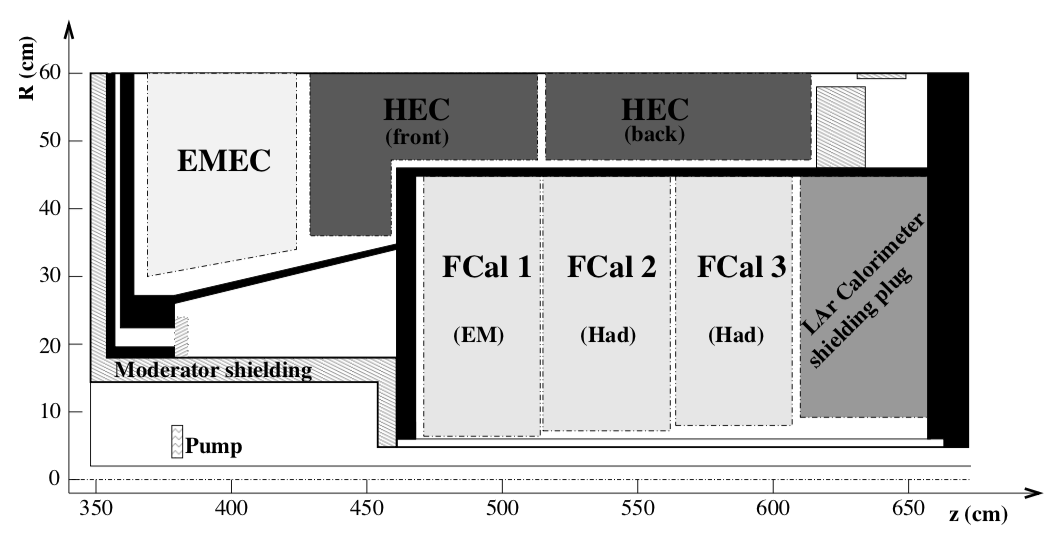
\includegraphics[width=0.65\textwidth]{figures/chapter2/calorimeters/atlas_fcal}
        \caption{
        }
        \label{fig:fcal}
    \end{center}
\end{figure}
